\documentclass{article}
\usepackage{CJKutf8}
\usepackage{graphicx}
\usepackage{subfigure}
\usepackage{listings}
\usepackage[colorlinks,linkcolor=blue]{hyperref}
\usepackage{ulem}
\usepackage{xcolor}
\usepackage{caption2}
\usepackage{amssymb}

\title{Latex Demo}
\author{hoochanlon}
\date{\today}

\begin{document}
	\begin{CJK*}{UTF8}{gbsn}
		\maketitle
		\tableofcontents

		% 强制分隔新起一页
		\clearpage
		\section*{测试:* 表示不带编号的部分}
		lorem ipsum dolor sit amet, consectetuer adipiscing elit.Ut purus elit,vestibulum ut, placerat ac,
		adipiscing vitae,felis. Curabitur dictum gravida mauris.lorem ipsum dolor sit amet, consectetuer,lorem i
		psum dolor sit amet, consectetuer adipiscing elit.Ut purus elit,vestibulum ut, placerat ac.

		回车两次代表换行,以及测试效果。
		\setlength{\parskip}{1em}

		看看 \verb| \setlength{\parskip}{1em} | 设置间距的效果。\\ \\
		两个 \verb| \\ | 代表换行,以及测试效果。 \\
		这是一条直线:\hrulefill \\
		这是一条虚线:\dotfill

		说明文字部分,设置文字链接: \href{http://www.baidu.com/}{百度}。另外,换行文字对齐问题:

		测试效果 \par
		效果测试\par

		\begin{flushleft}
		现在开始,可通过 \verb| begin{flushleft} | 进行控制。 \par
		图片可用 \verb| \ref{teaser} | 进行关联,如:图:\ref{teaser}所示。有关emoji,需要lualatex环境的支持。

		\begin{enumerate}
			\item CJKutf8:使得可以在LaTeX中直接输入中文,提供对中文的支持。
			\item graphicx:提供了插入图片的功能。
			\item subfigure:提供了创建并管理子图的功能,可以在一个浮动环境中插入多个子图,并进行编号和引用。
			\item listings:用于在LaTeX中排版源代码,提供了一套灵活的排版设置,可以高亮显示不同编程语言的关键字和语法。
			\item hyperref:用于添加超链接和书签,可以生成可点击的链接,如网址、目录等。
			\item ulem:提供了一系列修饰文本的命令,如下划线、波浪线、删除线等。
			\item xcolor:扩展了颜色的功能,提供了更多的颜色模型和定义颜色的方式。
			\item caption2:修改和自定义标题的样式,如字体、间距等。
			\item amssymb:提供了一系列额外的数学符号,如各种数学字体、特殊符号等。
		\end{enumerate}

		\end{flushleft}

		\clearpage
		\section{插入图片}
		这里插入一张网络图片:h: here; t: top; b: bottom; p: page of float。
		\renewcommand{\figurename}{图} % 将图表的标题设置为中文“图”
		\begin{figure}[htbp]
			\centering
			\subfigure[场景1]{
				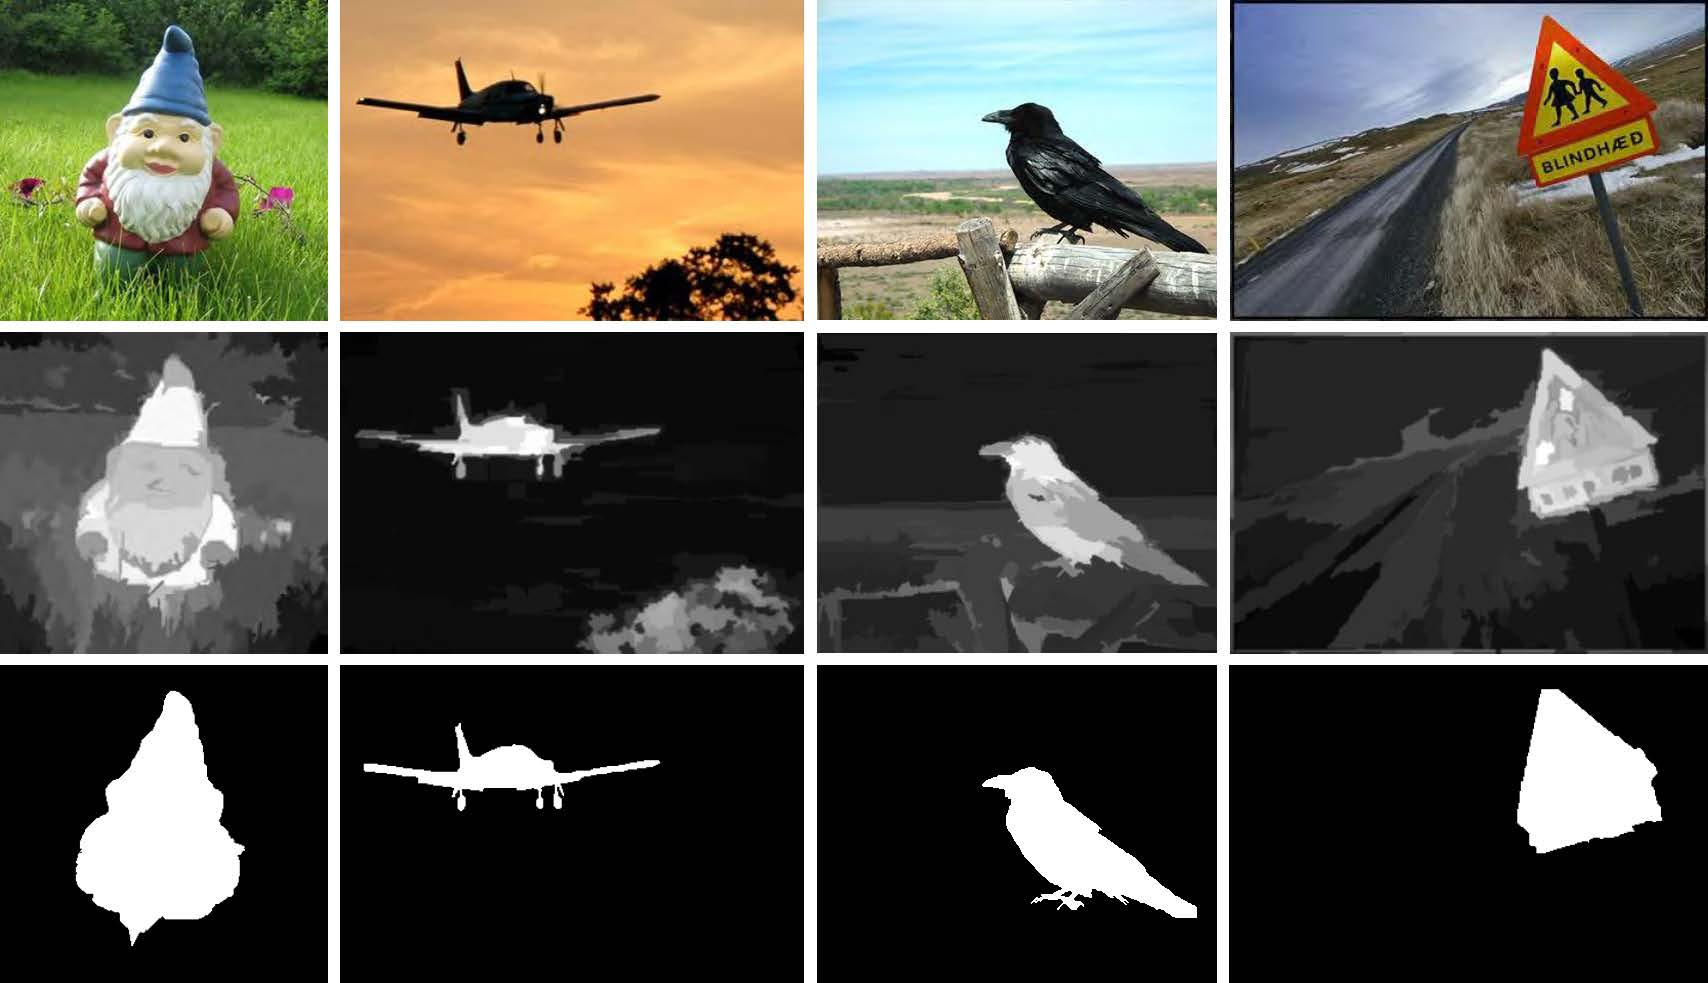
\includegraphics[width=0.4\textwidth]{./figures/teaser.jpg}
				\label{teaser}
			}
			\subfigure[场景2]{
				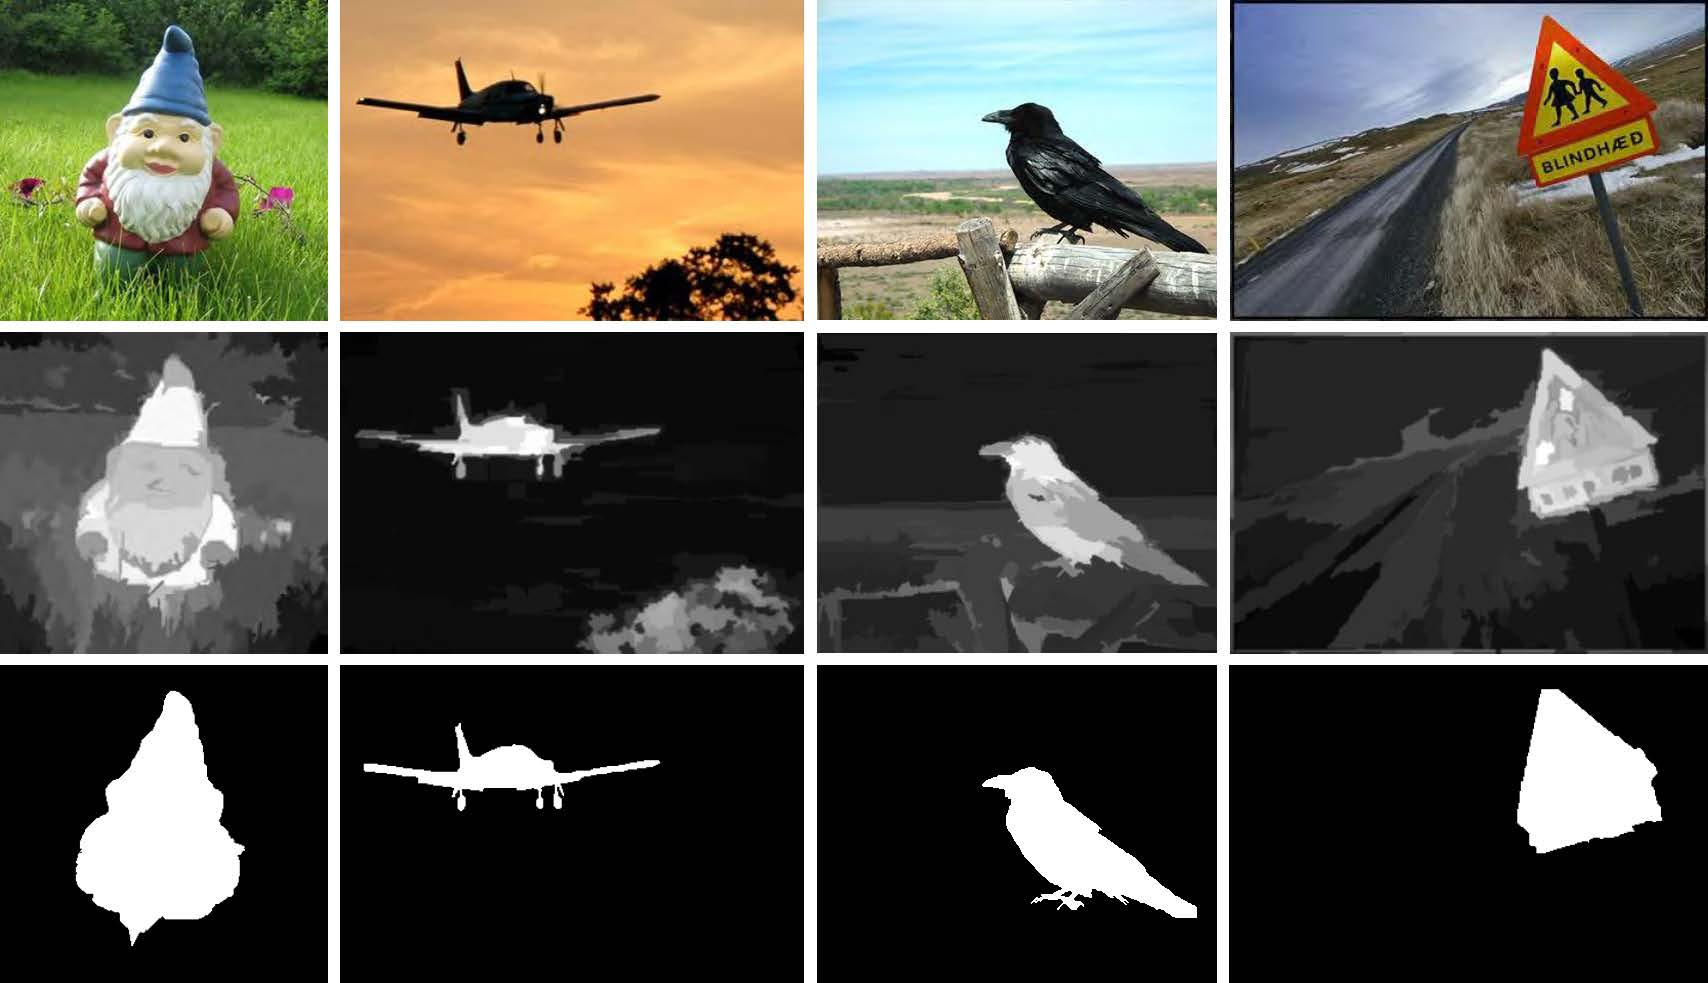
\includegraphics[width=0.4\textwidth]{./figures/teaser.jpg}
			}
			\centering
			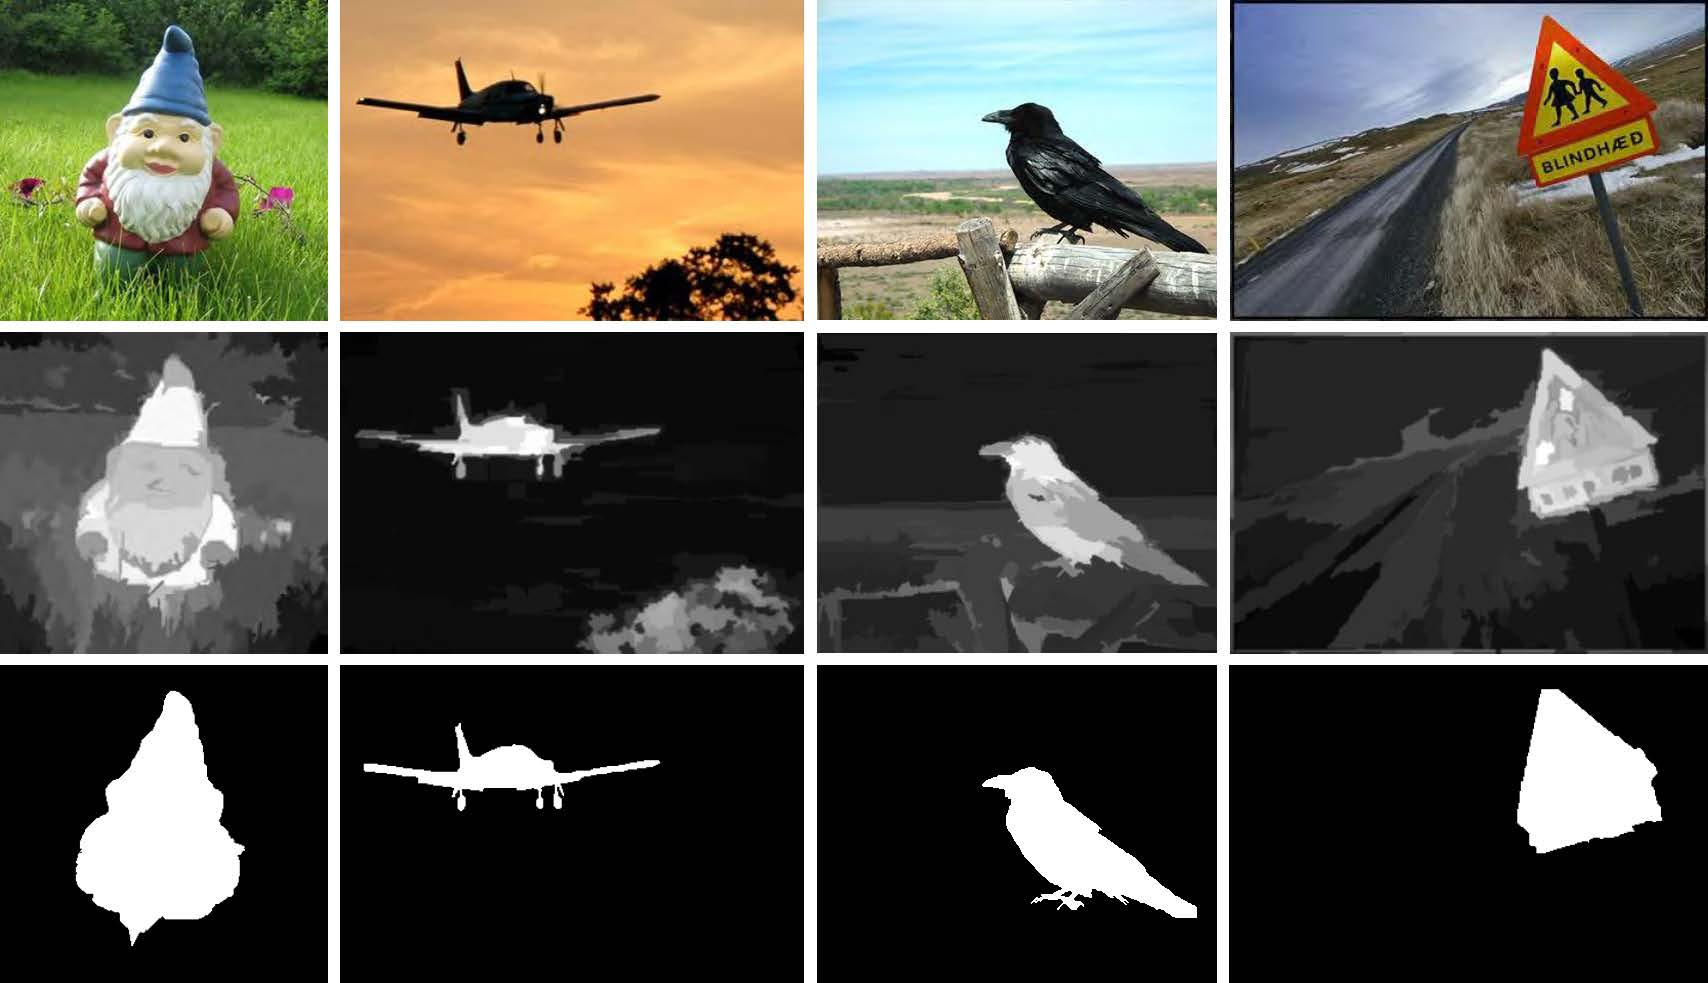
\includegraphics[width=0.6\textwidth]{./figures/teaser.jpg}
			\caption{这是图片}
		\end{figure}

		% 设置标题与图片之间的间距为10pt

		\begin{figure}[htbp]
			\centering
			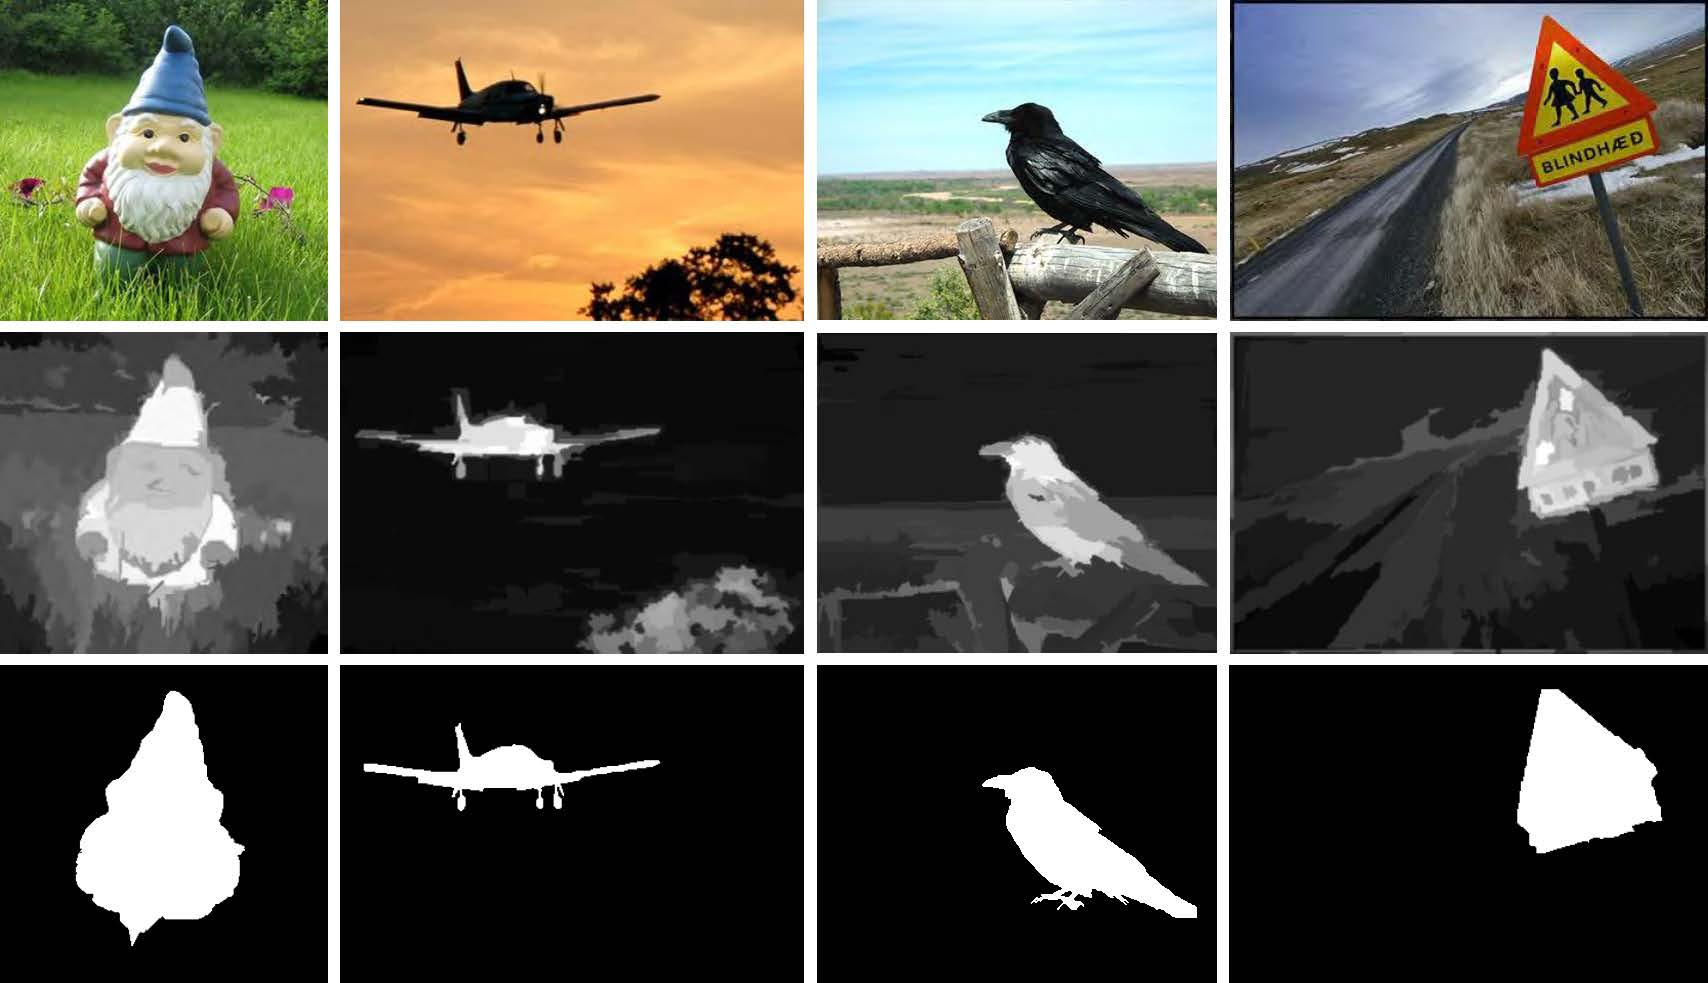
\includegraphics[width=0.6\textwidth]{./figures/teaser.jpg}
			\caption{这是图片的标题}
		\end{figure}


		\clearpage
		\section{字体样式}
		\setlength{\parskip}{1em}
		\subsection{第一小节}
		\begin{flushleft}

		文字样式:粗体、下划线、删除线、上标、下标、脚注

		\textbf{粗体文本} ~ \textmd{中等粗细} \par
		\uline{下划线文本} ~ \sout{删除线文本} \par
		$x^2$  上标 ~ $H_2O$ 下标 \par

		这是一个带有脚注的句子。\footnote{这是脚注的内容。}
		还可以在同一个段落中添加多个脚注。\footnote{第一个脚注。} \footnote{第二个脚注。}

		\subsection{字体大小、颜色、背景色}
		\Large 这是大号字体文本 \par
		设置的同时也会造成局部影响。\par
		\normalsize 这是正常大小字体文本 \par
		\textsf{无衬线字体} \textcolor{blue}{蓝色文本} \par
		\texttt{等宽字体} \colorbox{yellow}{黄色背景的文本} \par

		\end{flushleft}

		\clearpage
		\section{数学与希腊符号表}
		\begin{flushleft}
		$\alpha$ 可以输入 \verb | $\alpha$ | 生成希腊字母,以此类推。 \par
		$\int$ 可以输入 \verb | $\int$ | 生成积分符号。 \par
		$\sum$ 可以输入 \verb | $\sum$ | 生成求和符号。 \par
		$\prod$ 可以输入 \verb | $\prod$ | 生成乘积符号。 \par
		$\lim$ 可以输入 \verb | $\lim$ | 生成极限符号。 \par
		$\infty$ 可以输入 \verb | $\infty$ | 生成无穷符号。 \par
		$\partial$ 可以输入 \verb | $\partial$ | 生成偏微分符号。 \par
		$\nabla$ 可以输入 \verb | $\nabla$ | 生成 nabla 符号。 \par
		$\forall$ 可以输入 \verb | $\forall$ | 生成全称量词符号。 \par
		$\exists$ 可以输入 \verb | $\exists$ | 生成存在量词符号。 \par
		$\neg$ 可以输入 \verb | $\neg$ | 生成非逻辑符号。 \par
		$\in$ 可以输入 \verb | $\in$ | 生成属于符号。 \par
		$\notin$ 可以输入 \verb | $\notin$ | 生成不属于符号。 \par
		$\subset$ 可以输入 \verb | $\subset$ | 生成真子集符号。 \par
		$\subseteq$ 可以输入 \verb | $\subseteq$ | 生成子集符号。 \par
		$\cup$ 可以输入 \verb | $\cup$ | 生成并集符号。 \par
		$\cap$ 可以输入 \verb | $\cap$ | 生成交集符号。 \par
		$\Rightarrow$ 可以输入 \verb | $\Rightarrow$ | 生成蕴含符号。 \par
		$\Leftrightarrow$ 可以输入 \verb | $\Leftrightarrow$ | 生成等价符号。 \par
		$\to$ 可以输入 \verb | $\to$ | 生成箭头符号。 \par
		$\mapsto$ 可以输入 \verb | $\mapsto$ | 生成映射符号。 \par
		$\sim$ 可以输入 \verb | $\sim$ | 生成相似符号。 \par
		$\simeq$ 可以输入 \verb | $\simeq$ | 生成近似符号。 \par
		$\approx$ 可以输入 \verb | $\approx$ | 生成约等于符号。 \par
		$\neq$ 可以输入 \verb | $\neq$ | 生成不等于符号。 \par
		$\equiv$ 可以输入 \verb | $\equiv$ | 生成恒等符号。 \par
		$\leq$ 可以输入 \verb | $\leq$ | 生成小于等于符号。 \par
		$\geq$ 可以输入 \verb | $\geq$ | 生成大于等于符号。 \par
		$\pm$ 可以输入 \verb | $\pm$ | 生成正负号。 \par
		$\times$ 可以输入 \verb | $\times$ | 生成乘号。 \par
		$\div$ 可以输入 \verb | $\div$ | 生成除号。 \par
		$\cdot$ 可以输入 \verb | $\cdot$ | 生成点乘符号。 \par
		$\circ$ 可以输入 \verb | $\circ$ | 生成圆圈符号。 \par
		$\perp$ 可以输入 \verb | $\perp$ | 生成垂直符号。 \par
		$\parallel$ 可以输入 \verb | $\parallel$ | 生成平行符号。 \par
		$\angle$ 可以输入 \verb | $\angle$ | 生成角符号。 \par
		$\triangle$ 可以输入 \verb | $\triangle$ | 生成三角符号。 \par
		由于 $a = b$,$\because a + c = b + c$。\\
		所以,$\therefore a + c$ 等于 $b + c$。
		\end{flushleft}

	\end{CJK*}
\end{document}
